\documentclass[a4paper, 12pt]{article}
\usepackage[utf8x]{inputenc}
\usepackage{cmap}
\usepackage[english, russian]{babel}
\usepackage{indentfirst}
\usepackage[left=20mm, top=20mm, right=20mm, bottom=20mm]{geometry}
\usepackage{tikz}
\usepackage{float}
\usepackage{amsmath, amsfonts, amssymb}
\usepackage{graphicx}
\usepackage{fancybox, fancyhdr}
\usepackage{hyperref}
\usepackage{listings}
\usepackage{caption}
\usepackage{subcaption}
\usepackage{xcolor}
\usepackage{paralist}
\usepackage{matlab-prettifier}
\pagestyle{fancy}
\fancyhf{}
\fancyhead[L]{Лабораторная работа №5}
\fancyhead[R]{Моделирование динамических систем}
\fancyfoot[C]{\thepage}
\graphicspath{{images/}}
\usetikzlibrary{patterns}
\definecolor{LightGray}{gray}{0.95}
\definecolor{LightGray2}{gray}{0.7}
\lstset{
    style=Matlab-editor,
    basicstyle=\mlttfamily,
    numbers=left,
    numberstyle=\scriptsize\color{gray},
    stepnumber=1,
    numbersep=5pt,
    frame=single,
    rulecolor=\color{LightGray2},
    backgroundcolor=\color{LightGray},
    breaklines=true,
    showstringspaces=false
}
\hypersetup{
    colorlinks=true,
    linkcolor=blue,
    filecolor=magenta,
    urlcolor=cyan,
    pdftitle={contents setup},
    pdfpagemode=FullScreen,
}
\setlength{\parskip}{1.5mm}
\setlength{\headheight}{15pt}
\setlength{\footskip}{15pt}
\allowdisplaybreaks
\DeclareMathOperator{\sinc}{sinc}

\begin{document}
    \begin{titlepage}

        \begin{center}
        
\includegraphics[width=0.3\textwidth]{itmo.png}
        \vfill
        
        Федеральное государственное автономное образовательное учреждение высшего образования
        «Национальный Исследовательский Университет ИТМО»\\
            
        \vfill
        {\large\bf ЛАБОРАТОРНАЯ РАБОТА №5}\\
        {\large\bf ПРЕДМЕТ «МОДЕЛИРОВАНИЕ ДИНАМИЧЕСКИХ СИСТЕМ»}\\
        {\large\bf ТЕМА «СИСТЕМЫ С ЗАДЕРЖКАМИ»}\\
        Вариант 4
        \vfill

        \begin{flushright}
            \begin{minipage}{.45\textwidth}
            {
                \hbox{Преподаватель:}
                \hbox{Семенов Д. М.}
                \hbox{}
                \hbox{Выполнили:}
                \hbox{Румянцев А. А., 368731}
                \hbox{Дьячихин Д. Н., 339080}
                \hbox{Овчинников П. А., 368606}
                \hbox{}
                \hbox{Факультет: СУиР}
            }
            \end{minipage}
        \end{flushright}
        
        \vfill
                
        Санкт-Петербург\\
        2024
        \end{center}
    \end{titlepage}
    
    \tableofcontents

    \newpage
    \section{Задание 1}
    \subsection{Условие}
    Дана следующая система с задержкой: $$\dot{x}(t)=-\,\text{sign}(x(t-h)),\ \ t\geq0,\,h>0,$$
    где $$\text{sign}\,x=
    \begin{cases}
        1, & x>0,\\
        -1, & x<0,\\
        0, & x=0,
    \end{cases}$$
    $h=2$ -- постоянная задержка, $x(t)=\varphi(t)$ при $t\in[-h,0]$.


    Используя метод шагов, построить график решения системы при
    $$\varphi(t)=
    \begin{cases}
        -0.5, & t\in[-2,-1.5),\\
        t+1, & t\in[-1.5,0]
    \end{cases}
    $$


    \subsection{Выполнение}
    Ограничимся решением системы на интервале $[-2,2]$. \textit{Шаг 1}.
    $$
    t\in[0,2],\ \ x(0)=\varphi(0)=1,\ \dot{x}(t)=-\,\text{sign}(\varphi(t-2))\Rightarrow
    $$
    $$
    \Rightarrow\begin{cases}
        \dot{x}(t)=-1, & \varphi(t-2)>0,\\
        \dot{x}(t)=1, & \varphi(t-2)<0,\\
        x(t)=C, & \varphi(t-2)=0
    \end{cases}\Rightarrow
    $$
    $$
    \Rightarrow
    \begin{cases}
        \dot{x}=-1, & t\in(1,2]\\
        \dot{x}=1, & t\in(0,1]
    \end{cases}
    $$
    \textit{Шаг 1.1.}
    $$
    \dot{x}(t)=1,\ \ t\in(0,1],
    $$
    $$
    x(t)=\int1\,dt=t+C_1,\ \ x(0)=1\Rightarrow x(0)=0+C_1=1\Rightarrow C_1=1\Rightarrow x(t)=t+1
    $$
    Найдем $x(t)$ для следующего момента времени $t=1$:
    $$
    x(t=1)=1+1=2
    $$
    \textit{Шаг 1.2.}
    $$
    \dot{x}(t)=-1,\ \ t\in(1,2],
    $$
    $$
    x(t)=\int-1\,dt=-t+C_2,\ \ x(1)=2\Rightarrow x(1)=-1+C_2=2\Rightarrow C_2=3\Rightarrow x(t)=-t+3
    $$
    Найдем $x(t)$ для следующего момента времени $t=2$:
    $$
    x(t=2)=-2+3=1
    $$
    \textit{Шаг 2.}
    Теперь интервал $(h,2h]$
    $$
    t\in(2,4],\ \ x(2)=1,\ \dot{x}(t)=-\,\text{sign}(x(t-2))\Rightarrow
    $$
    $$
    \Rightarrow\begin{cases}
        \dot{x}(t)=-1, & x(t-2)>0,\\
        \dot{x}(t)=1, & x(t-2)<0,\\
        x(t)=C, & x(t-2)=0
    \end{cases}\Rightarrow
    \dot{x}(t)=-1,\ t\in(2,4]
    $$
    $$
    \dot{x}(t)=-1,\ \ t\in(2,4],
    $$
    $$
    x(t)=\int-1\,dt=-t+C_3,\ \ x(2)=1\Rightarrow x(2)=-2+C_3=1\Rightarrow C_3=3\Rightarrow x(t)=-t+3
    $$
    В итоге получаем
    $$
    x(t)=
    \begin{cases}
        t+1, & t\in(0,1],\\
        -t+3, & t\in(1,4]
    \end{cases}
    $$
    На рис. \ref{fig:task1} приведен график решения уравнения системы с задержкой.
    Программа для построения графика представлена на листинге \ref{task1code}.
    \begin{figure}[H]
        \centering
        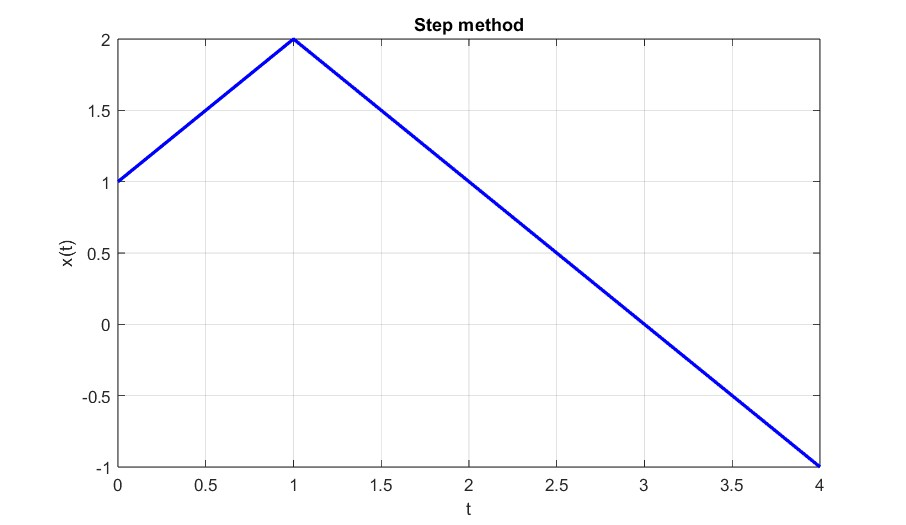
\includegraphics[scale=0.4]{task1.jpg}
        \captionsetup{skip=0pt}
        \caption{Решение уравнения системы с задержкой при $h=2$ методом шагов}
        \label{fig:task1}
    \end{figure}


    \section{Задание 2}
    \subsection{Условие}
    Дана система с некоторой произвольной задержкой $\tau(t)$:
    $$\dot{x}(t)=-3x(t)-0.2x(t-\tau(t))$$
    Построить функцию Ляпунова. С помощью метода Разумихина
    доказать устойчивость данной системы. 
    Для решения матричных неравенств использовать критерий Сильвестра.


    \subsection{Выполнение}
    Согласно методу Разумихина, система является
    асимптотически устойчивой, когда разрешимо линейное матричное
    неравенство (LMI):
    $$
    \psi=
    \begin{bmatrix}
        A^TP+PA+qP & PA_1\\
        A^T_1P & -qP
    \end{bmatrix}<0,\ \ q>0,\ P>0
    $$
    В общем виде линейная динамическая система с переменной задержкой имеет вид
    $$
    \dot{x}(t)=Ax(t)+A_1x(t-\tau(t)),\ \ t\geq t_0
    $$
    Исходя из нашего уравнения:
    $$
    \begin{matrix}
        A=-3\\
        A_1=-0.2
    \end{matrix}
    $$
    Подставим $A,A_1$ в элементы матрицы $\psi$ и упростим выражения:
    $$
    \begin{matrix}
        A^TP+PA+qP=-3P+P\cdot(-3)+qP=-P(6-q)\\
        PA_1=A^T_1P=-0.2P
    \end{matrix}
    $$
    Получим матричное неравенство
    $$
    \psi=
    \begin{bmatrix}
        -P(6-q) & -0.2P\\
        -0.2P & -qP
    \end{bmatrix}<0,\ \ q>0,\ P>0
    $$
    Неравенство верно тогда, когда выполняется критерий Сильвестра:
    $$
    \begin{cases}
        -P(6-q)<0,\\
        \det{\{\psi\}}=qP^2(6-q)-0.04P^2>0,\\
        q>0,\ P>0
    \end{cases}
    $$
    Рассмотрим первое неравенство (при условии третьего):
    $$-P(6-q)<0\Rightarrow6-q>0\Rightarrow0<q<6$$
    Рассмотрим второе неравенство:
    $$qP^2(6-q)-0.04P^2>0\Rightarrow q^2-6q+0.04<0\Rightarrow(q-0.007)(q-5.993)<0\Rightarrow0.007<q<5.993$$
    Получаем
    $$
    \begin{cases}
        0<q<6,\\
        0.007<q<5.993
    \end{cases}
    \Rightarrow
    0.007<q<5.993
    $$
    Таким образом, система LMI разрешима $\forall q\in(0.007,5.993)$, следовательно, система
    асимптотически устойчива.


    \section{Задание 3}
    \subsection{Условие}
    Дана система с постоянной задержкой $h$:
    $$\dot{x}(t)=Ax(t)+A_1x(t-h),$$ где $x\in\mathbb{R}^2$,
    $$
    A=
    \begin{bmatrix}
        -5 & -2\\
        1 & -2
    \end{bmatrix},\ \
    A_1=
    \begin{bmatrix}
        2 & 1\\
        0 & -1
    \end{bmatrix},\ \
    h=1
    $$
    \begin{compactitem}
        \item Промоделировать данную систему.
        \item С помощью функционала Ляпунова-Красовского доказать
        устойчивость данной системы.
    \end{compactitem}


    \subsection{Выполнение}
    Моделирование рассматриваемой системы представлено на рис. \ref{fig:task3}.
    Программа для построения графика представлена на листинге \ref{task3code1}.
    \begin{figure}[H]
        \centering
        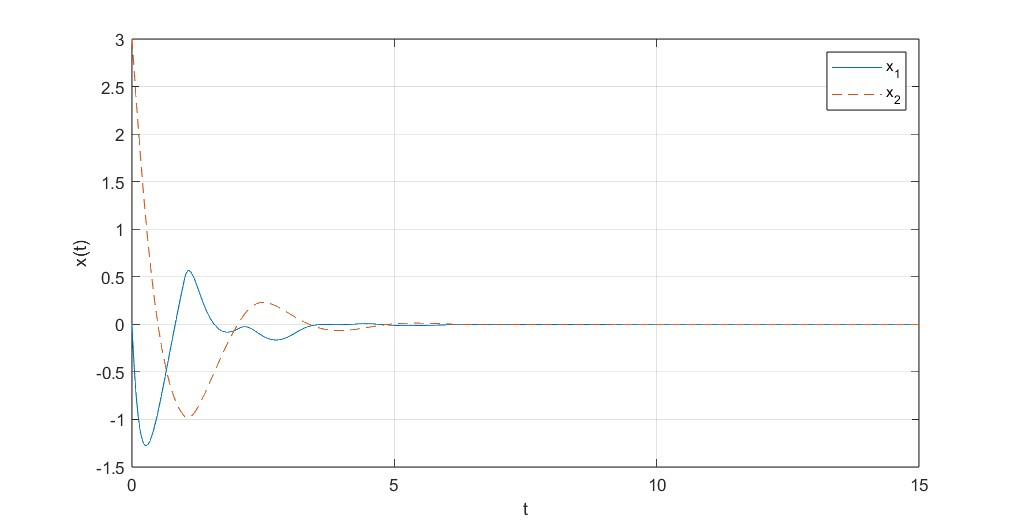
\includegraphics[scale=0.4]{task3.jpg}
        \captionsetup{skip=0pt}
        \caption{Моделирование системы с задержкой $h=1$}
        \label{fig:task3}
    \end{figure}


    Рассмотрим второй пункт. Для системы с задержкой решается матричное неравенство вида
    $$
    \psi=
    \begin{bmatrix}
        A^TP+PA+Q & PA_1\\
        A^T_1P & -(1-\dot{\tau}(t))Q
    \end{bmatrix}<0,\ \ Q>0,\, P>0
    $$
    Так как задержка $h=1$ постоянна, то $\dot{\tau}(t)=\dot{h}=1^{\prime}=0\Rightarrow1-\dot{\tau}(t)=1$.
    Имеем матричное неравенство
    $$
    \psi=
    \begin{bmatrix}
        A^TP+PA+Q & PA_1\\
        A^T_1P & -Q
    \end{bmatrix}<0,\ \ Q>0,\, P>0
    $$
    Проверим с помощью MATLAB программы, представленной на листинге \ref{task3code2}, решается
    ли матричное неравенство. Вывод результата проверки приведен на рис. \ref{fig:result3}.
    \begin{figure}[H]
        \centering
        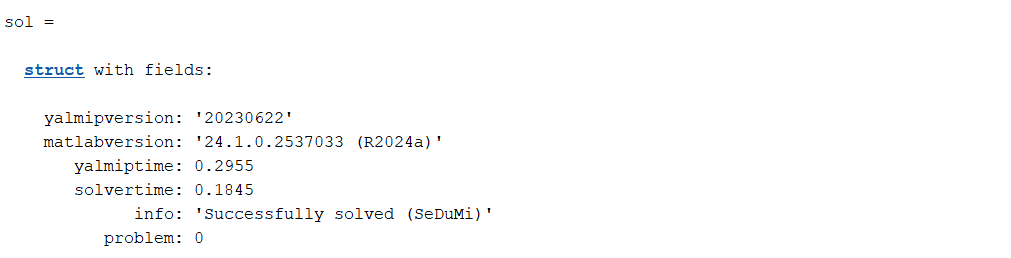
\includegraphics[scale=0.7]{result3.png}
        \captionsetup{skip=0pt}
        \caption{Вывод программы MATLAB}
        \label{fig:result3}
    \end{figure}
    \noindent Решение данного LMI в MATLAB дает следующий результат:
    $$
    P=
    \begin{bmatrix}
        0.2535 & 0.0247\\
        0.0247 & 0.5754
    \end{bmatrix},\ \
    Q=
    \begin{bmatrix}
        1.1341 & 0.0891\\
        0.0891 & 1.1561
    \end{bmatrix}
    $$
    Следовательно, данная система является устойчивой.


    \section{Вывод}
    В данной лабораторной работе мы решили систему с задержкой методом шагов и построили соответствующий график.
    Мы доказали устойчивость системы с некоторой произвольной задержкой, используя для решения матричных
    неравенств критерий Сильвестра. С помощью функционала Ляпунова-Красовского подтвердили устойчивость
    системы с постоянной задержкой, которую предварительно промоделировали.


    \section{Приложения}
    \begin{lstlisting}[label=task1code, caption={Программа для построения графика решения системы с задержкой методом шагов}]
    % Setting intervals
    t1 = 0:0.01:1; % Interval [0, 1]
    t2 = 1:0.01:4; % Interval [1, 4]

    % Calculate the function values at each interval
    x1 = t1 + 1;          % x(t) = t + 1 for t in [0, 1]
    x2 = -t2 + 3;         % x(t) = -t + 3 for t in [1, 4]

    % Combining intervals and values
    t = [t1, t2];         % Whole interval [0, 4]
    x = [x1, x2];         % Corresponding Function Values

    % Plotting a graph
    figure;
    plot(t, x, 'b', 'LineWidth', 2);
    grid on;
    xlabel('t');
    ylabel('x(t)');
    title('Step method');
    \end{lstlisting}


    \begin{lstlisting}[label=task3code1, caption={Программа для построения графика системы с задержкой}]
    %LabWork 5
    close all;

    h = 1; %delay
    MaxTime = 15;
    MinTime = 0;

    tspan = [0 MaxTime];
    tgrid = linspace(MinTime, MaxTime, 1000);

    % Solving
    control = false;
    sol = dde23(@ddefun, h, @history, tspan);
    x = deval(sol, tgrid);

    figure
    plot(tgrid, x(1,:));
    hold on
    grid on
    plot(tgrid, x(2,:), '--');
    legend('x_1','x_2');
    xlabel('t');
    ylabel('x(t)');



    function dxdt = ddefun(t, x, Z)
    A = [-5 -2; 1 -2];
    A1 = [2 1; 0 -1];

    dxdt = zeros(2,1);
    dxdt = A*x + A1*Z;
    end

    function phi = history(t)
    phi = zeros(2,1);
    phi(1,1) = 5*sin(t);
    phi(2,1) = 2*cos(t)+1;
    end
    \end{lstlisting}


    \begin{lstlisting}[label=task3code2, caption={Программа для проверки разрешимости матричных неравенств}]
    clc;
    clear all;

    A=[-5 -2; 1 -2];
    A1=[2 1; 0 -1];
    n=2;            

    P=sdpvar(n);   
    Q=sdpvar(n);
    TH=blkvar;       
    TH(1,1)=A'*P+P*A+Q;
    TH(1,2)=P*A1;
    TH(2,2)=-Q;
    TH=sdpvar(TH);


    F=[TH<=-0.0001,P>=0.0001,Q>=0.0001];
    %Setting the settings
    options=sdpsettings('solver','sedumi','verbose',0);
    %Solving the problem
    sol=optimize(F)
    %In the command window we get information about
    %whether the given matrix inequalities are solvable.
    %In this case we have: "info: 'Successfully solved
    %(SeDuMi-1.3)'". This means that the system of matrix
    %inequalities is solvable, and the original system is stable.
    P_value = value(P);
    Q_value = value(Q);

    disp('Matrix P:');
    disp(P_value);

    disp('Matrix Q:');
    disp(Q_value);
    \end{lstlisting}
\end{document}